\documentclass{article}
\usepackage{tikz}
\usetikzlibrary{arrows.meta,positioning,calc,shapes.geometric}
\pagestyle{empty}
\begin{document}
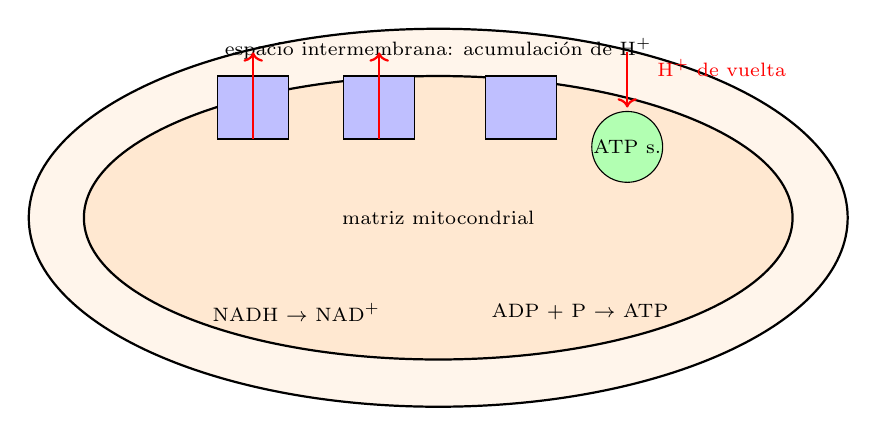
\begin{tikzpicture}

\draw[thick, fill=orange!8] (0,0) ellipse (5.2 and 2.4); \draw[thick, fill=orange!18] (0,0) ellipse (4.5 and 1.8);
\node[font=\scriptsize] at (0,0.0) {matriz mitocondrial};
\node[font=\scriptsize] at (0,2.15) {espacio intermembrana: acumulación de H$^+$};
\foreach \x in {-2.8,-1.2} {\draw[fill=blue!25] (\x,1.0) rectangle (\x+0.9,1.8); \draw[->, thick, red] (\x+0.45,1.0) -- (\x+0.45,2.1);}
\draw[fill=blue!25] (0.6,1.0) rectangle (1.5,1.8);
\draw[fill=green!30] (2.4,0.9) circle (0.45); \node[font=\scriptsize] at (2.4,0.9) {ATP s.};
\draw[->, thick, red] (2.4,2.1) -- (2.4,1.4); \node[font=\scriptsize, red] at (3.6,1.9) {H$^+$ de vuelta};
\node[font=\scriptsize] at (-1.8,-1.2) {NADH $\to$ NAD$^+$}; \node[font=\scriptsize] at (1.8,-1.2) {ADP + P $\to$ ATP};

\end{tikzpicture}
\end{document}
